\documentclass[10pt,a4paper,twocolumn]{article}

\usepackage[T1]{fontenc} % extended font encoding
\usepackage{enumerate} % lists
\renewcommand{\familydefault}{\sfdefault} % sans-serif
\usepackage{microtype} % better text justification
\usepackage{graphicx} % allow including pictures
\usepackage{color} % colors for pictures
\usepackage{fancyhdr} % headers and footers
\usepackage{titling} % picture in the title
\usepackage{hyperref} % clickable links
\usepackage[left=2cm,right=2cm,top=3cm,bottom=3cm]{geometry} % wider and taller page

\pagenumbering{gobble} % hide page numbers
\setlength{\columnsep}{1cm} % space between columns
\setlength{\parskip}{\baselineskip} % paragraphs divided by empty lines
\setlength{\parindent}{0pt}

\pdfinfo{
   /Author (Zlosynth Instruments)
   /Title  (Achordion - Build Manual)
}

\pretitle{%
  \begin{center}
  \Huge
}
\posttitle{%
  \\
  \vspace{2cm}
  
\includegraphics[width=14cm]{schema.pdf}
  \end{center}
}

\begin{document}

\title{Achordion -- Build Manual}
\author{}
\date{}

\maketitle

\section{Overview}

You can always find the latest version of this build manual on
\url{https://zlosynth.com/achordion/build-manual.pdf}.

This kit contains 3 printed circuit boards (PCBs) with all the SMD parts already
pre-soldered. The through-hole components are left to be assembled by you.

Pay attention to the orientation and position of all the parts. Desoldering
them would be difficult and would probably break the module.

Two of the bigger PCBs have both sides labeled with a number and a letter. This
marking is referenced across this manual. The smaller yellow PCB, containing the
digital processing power, is referred to as Daisy Seed.

\newpage

\section{Tools required}

\begin{itemize}
  \item Soldering iron
  \item Masking tape
  \item Small flat head screwdriver
  \item Phillips head screwdriver
  \item Side-cutters
\end{itemize}

\newpage

\section{Bill of materials}

Start by unpacking all baggies into a bowl, so you don't lose any components.

\begin{tabular}{@{}rl@{}}
  1 \texttimes & Front panel \\
  1 \texttimes & PCB 1 \\
  1 \texttimes & PCB 2 \\
  1 \texttimes & Daisy Seed \\
  4 \texttimes & Potentiometer, M7 nut and washer \\
  1 \texttimes & Big knob \\
  3 \texttimes & Small knob \\
  7 \texttimes & 3.5mm jack socket, M6 nut and washer \\
  1 \texttimes & Tactile switch \\
  8 \texttimes & Red LED \\
  1 \texttimes & Hex standoff \\
  2 \texttimes & M3 screw \\
  1 \texttimes & Shrouded male connector 2\texttimes5 \\
  2 \texttimes & Female connector 1\texttimes20 \\
  1 \texttimes & Male connector 2\texttimes6 \\
  1 \texttimes & Female connector 2\texttimes6 \\
  1 \texttimes & Male connector 2\texttimes8 \\
  1 \texttimes & Female connector 2\texttimes8 \\
  1 \texttimes & Male connector 1\texttimes5
\end{tabular}

\begin{figure}[p]
  \centering
  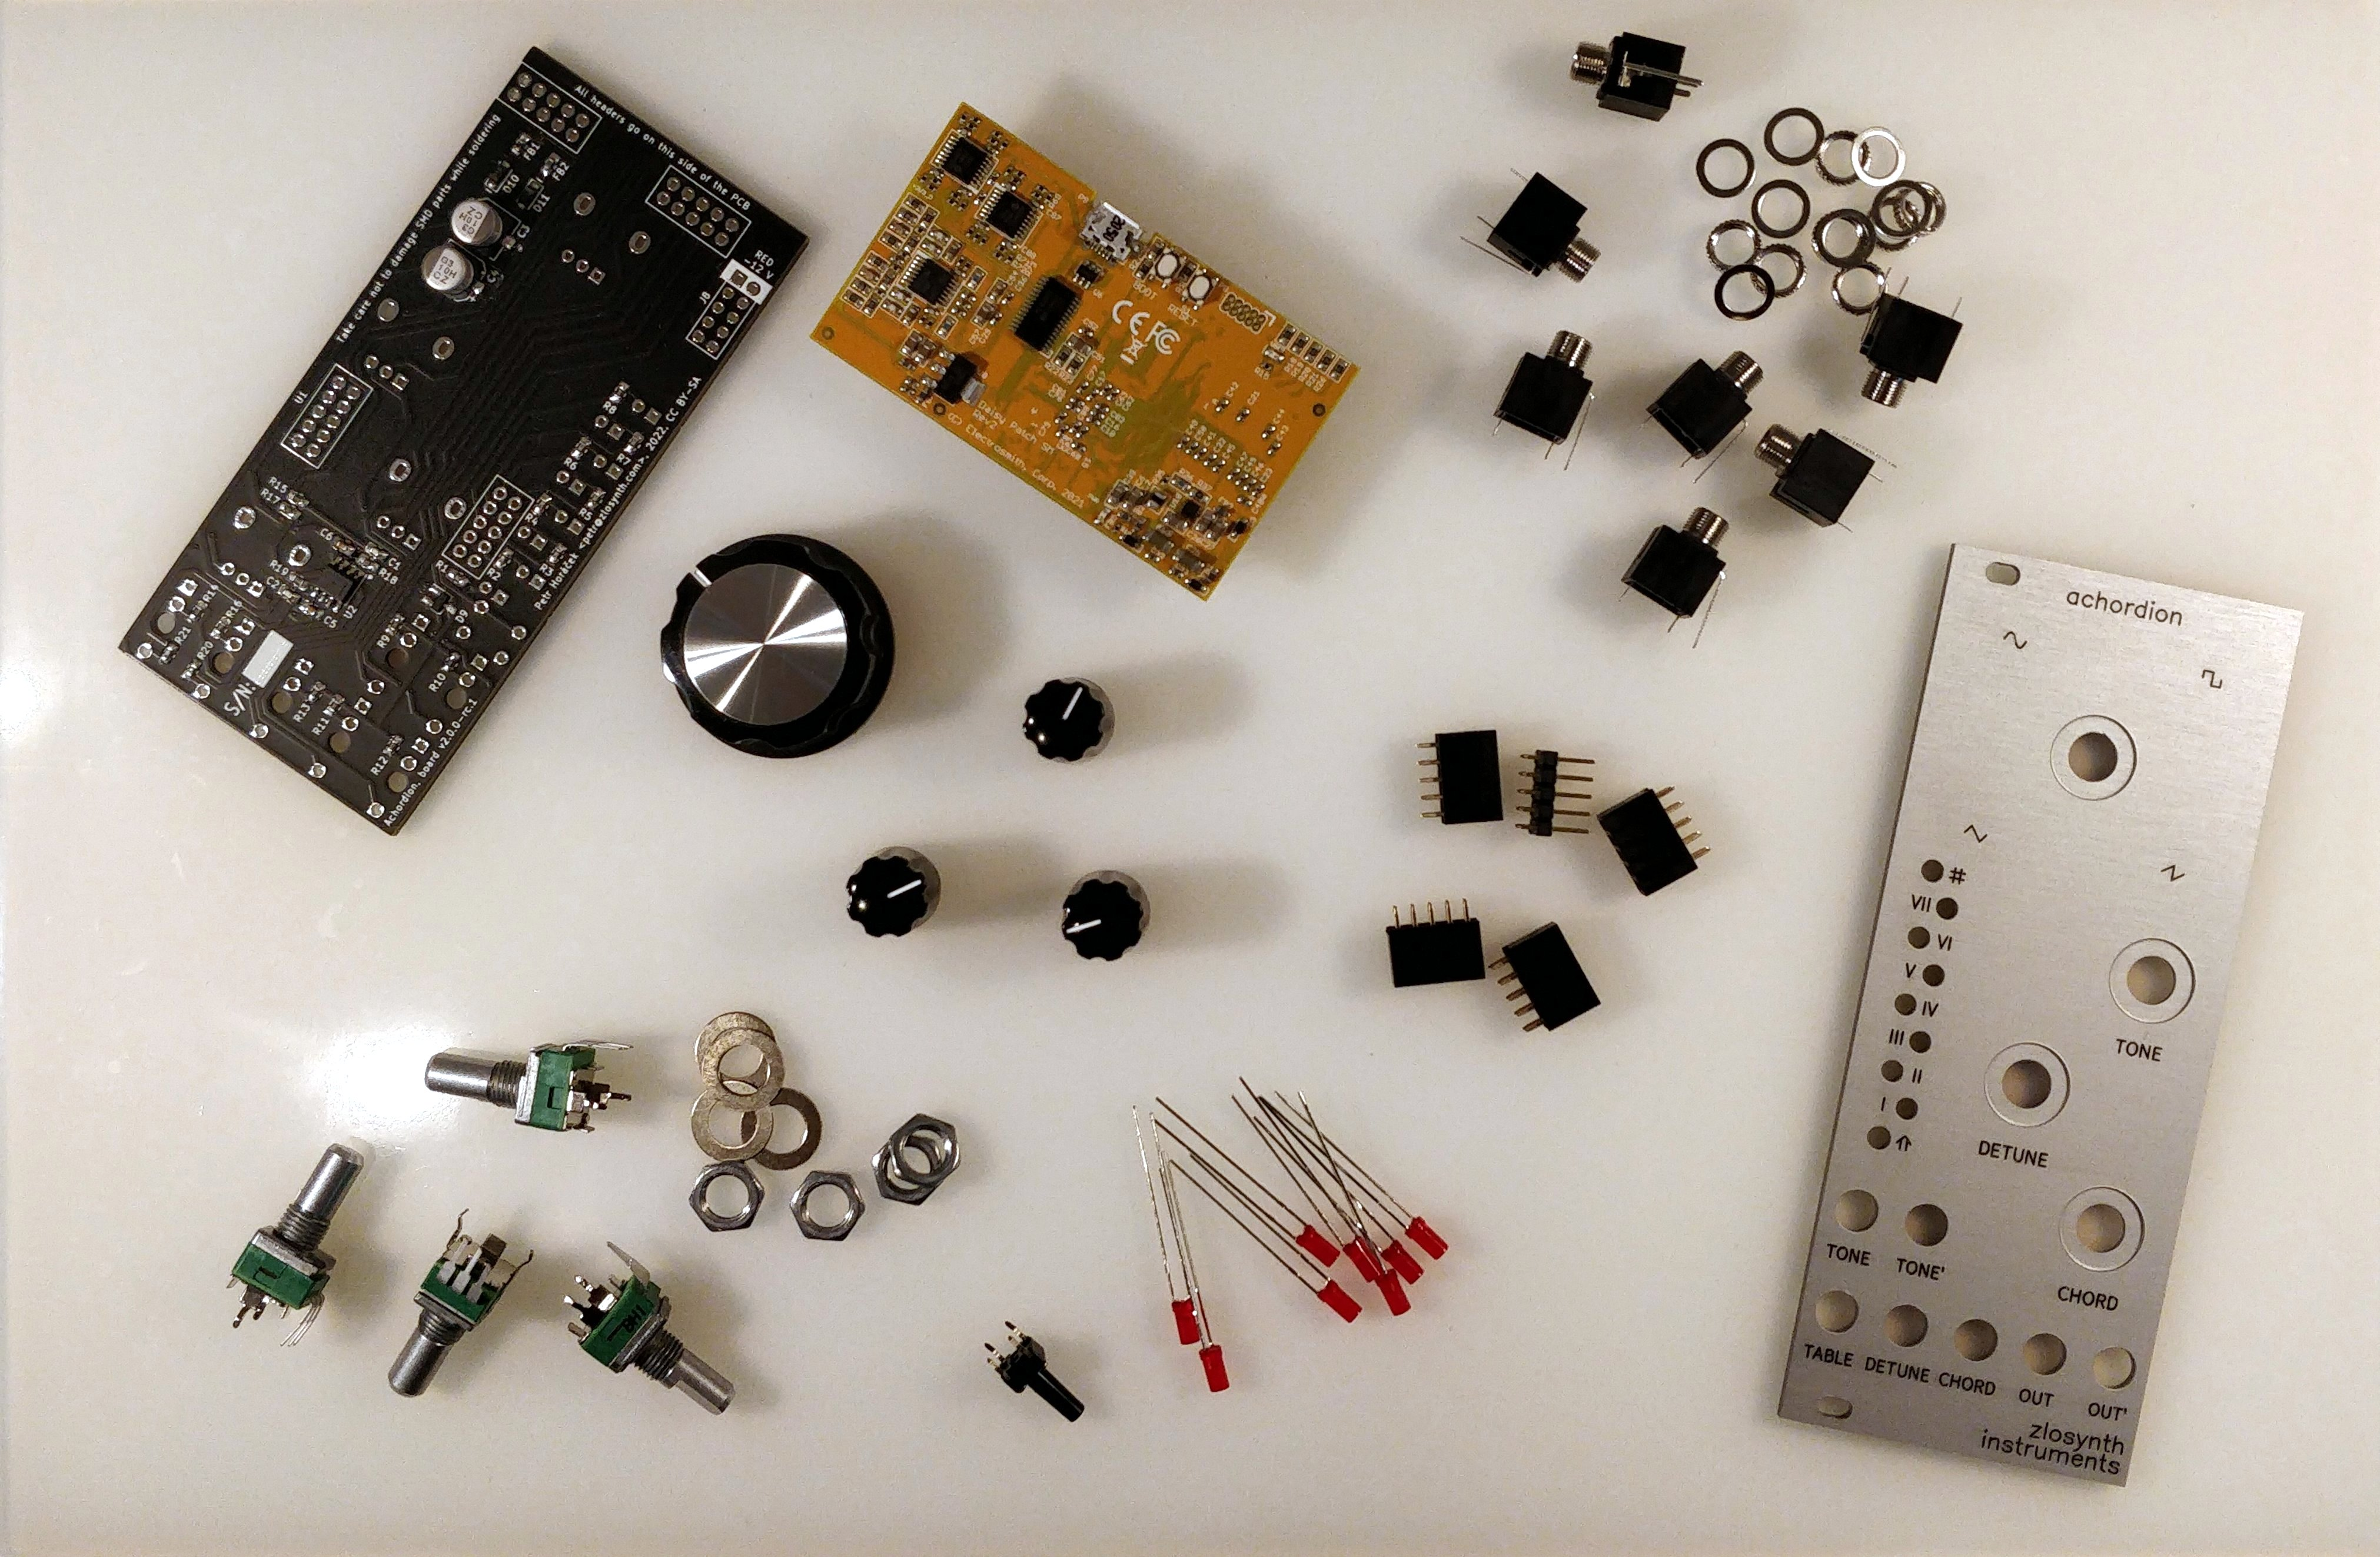
\includegraphics[width=\linewidth]{p01.jpg}
  \caption{All the components laid out}
\end{figure}

\section{PCB connectors}

The two bigger PCBs are connected with two pairs of connectors. To keep them
from wiggling, they are also secured with a standoff. See figures \ref{pcb1}
and \ref{pcb2}.

\begin{enumerate}
  \item Tighten the standoff with a screw to the PCB 1, it should be standing on the side 1B.
  \item Take the 2\texttimes6 and 2\texttimes8 connectors and join their male and female counterparts together.
  \item Put these connectors in the PCB 1, with the female part standing on the side 1B.
  \item Mount the PCB 2 on the connectors coming out from PCB 1 and align the two boards.
  \item Tighten the other side of the standoff with a screw. Securing the two boards with the standoff will make it easier to solder the connectors.
  \item Solder the connectors on both PCBs. Once this is done, unscrew the standoff and detach the PCBs.
\end{enumerate}

\begin{figure}[p]
  \centering
  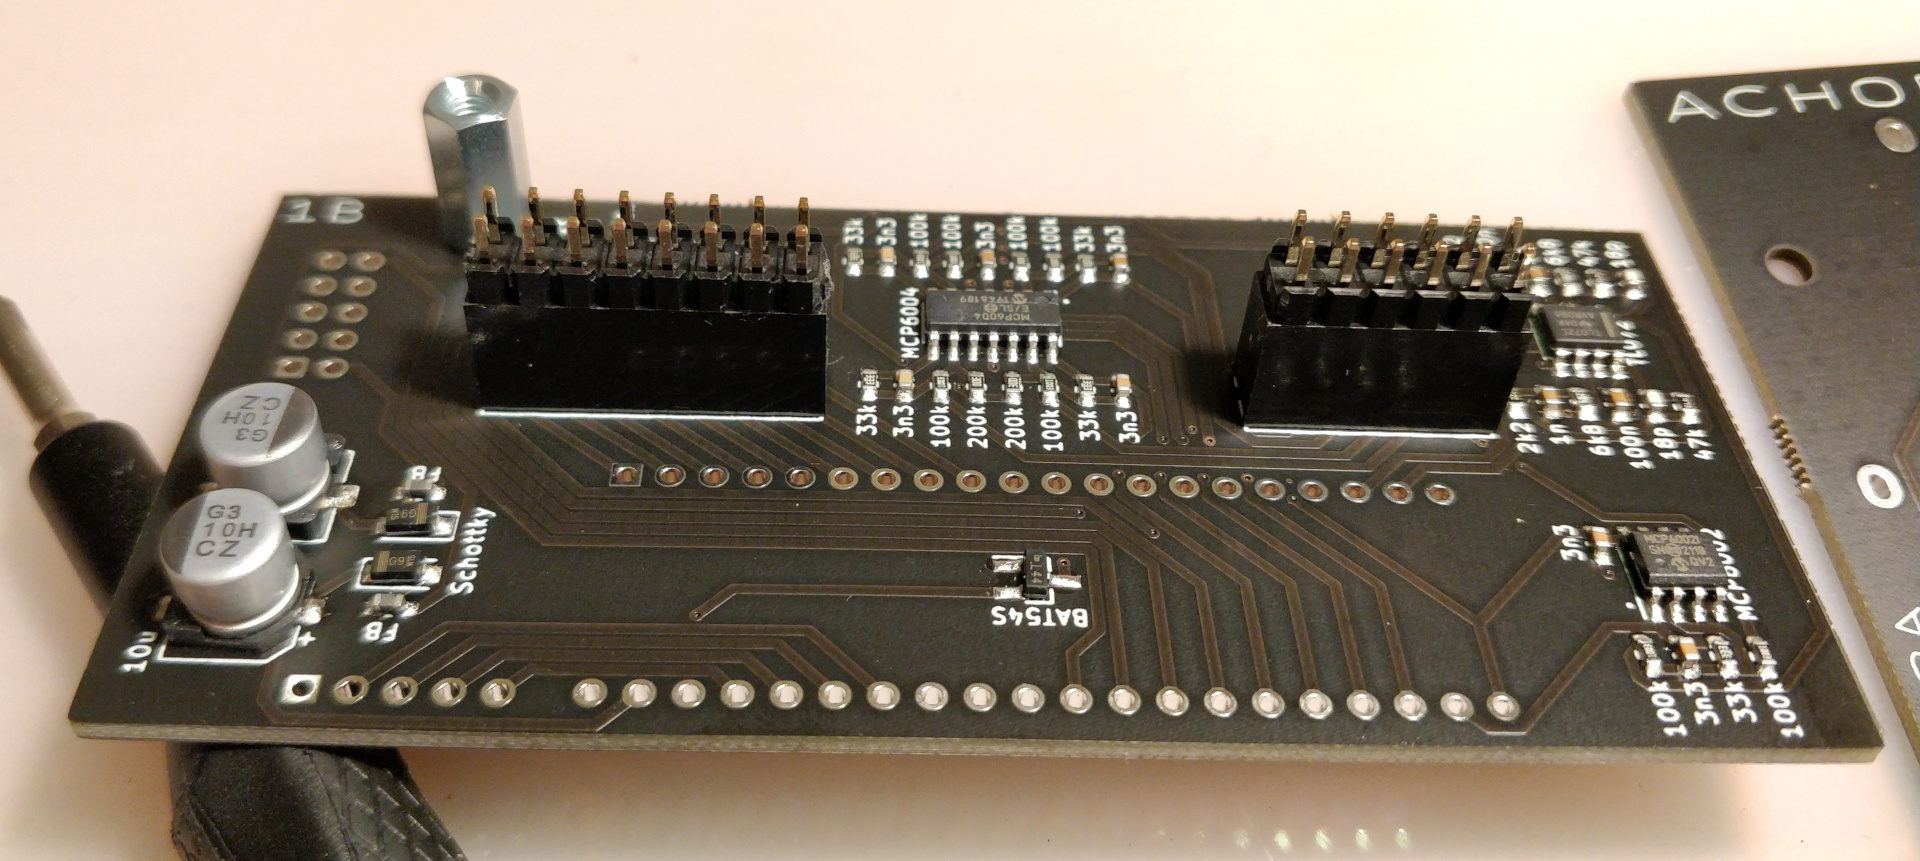
\includegraphics[width=\linewidth]{p02.jpg}
  \caption{PCB 1 with placed connectors and a standoff}
  \label{pcb1}
\end{figure}

\begin{figure}[p]
  \centering
  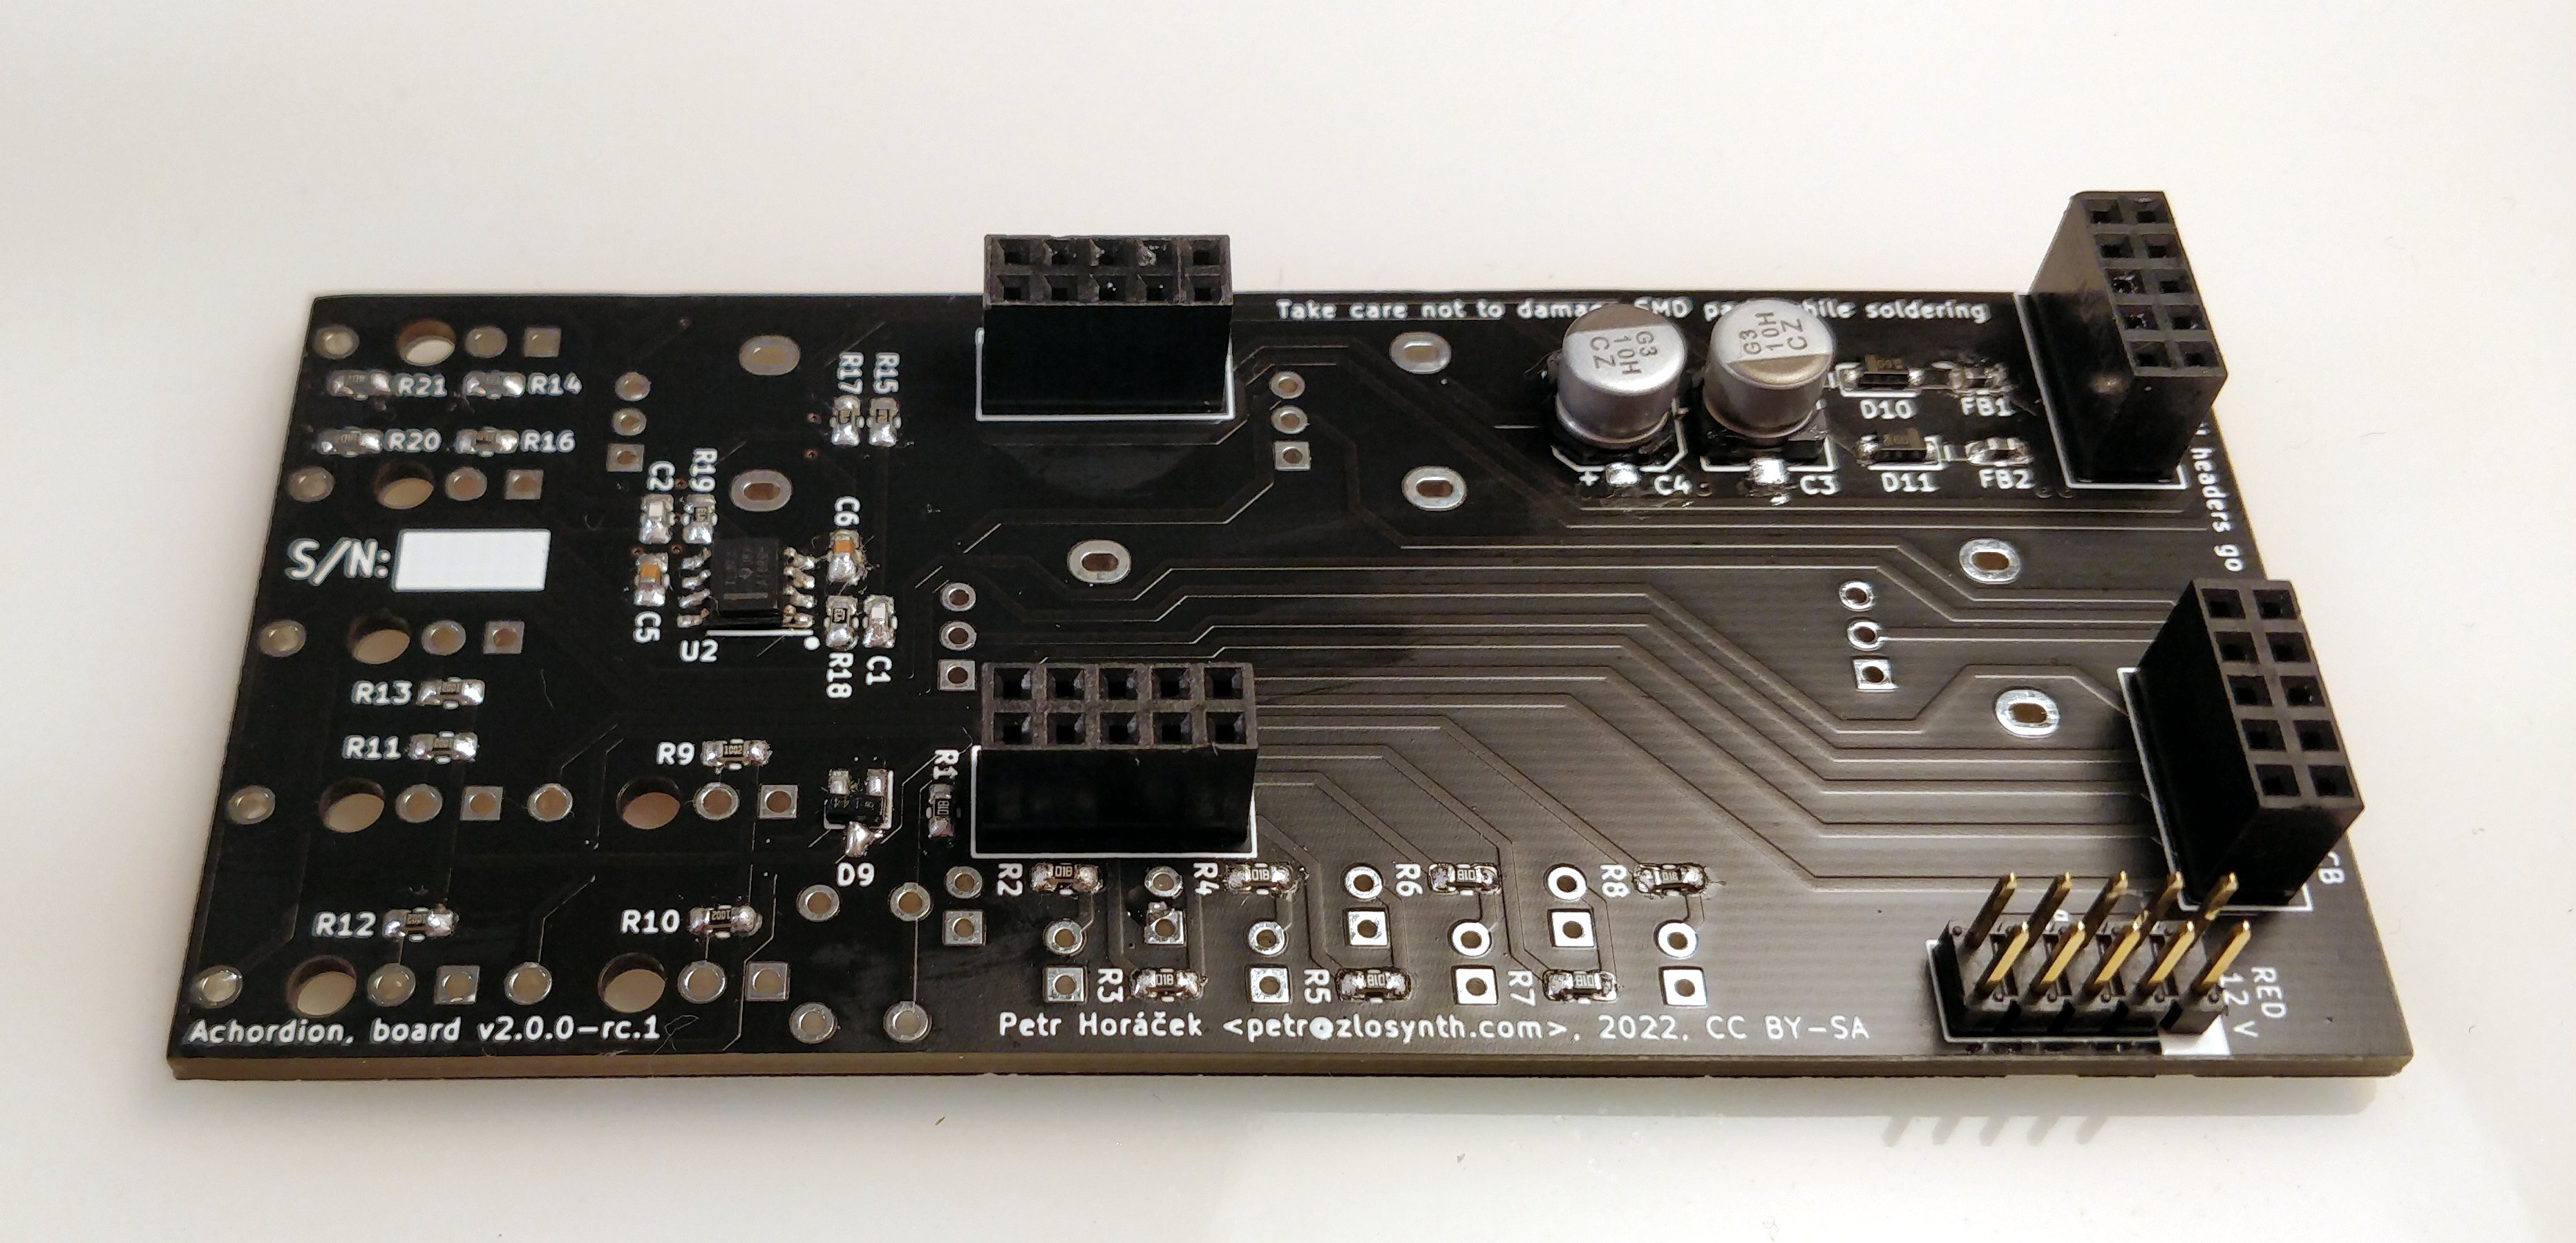
\includegraphics[width=\linewidth]{p03.jpg}
  \caption{PCB 2 placed on inter-board connectors}
  \label{pcb2}
\end{figure}

\clearpage

\section{Daisy Seed}

Daisy Seed is mounted on the PCB 1 with a set of connectors.

\begin{enumerate}
  \item Plug the two 1\texttimes20 female connectors on the pins of Daisy Seed. See figure \ref{daisy}.
  \item Place it in the PCB on the side 1A. The side on which Daisy Seed should have its USB connector is marked on the PCB.
  \item Solder all the pins in. Once done, detach Daisy Seed to prevent it from getting damaged while progressing with the build.
\end{enumerate}

\begin{figure}[p]
  \centering
  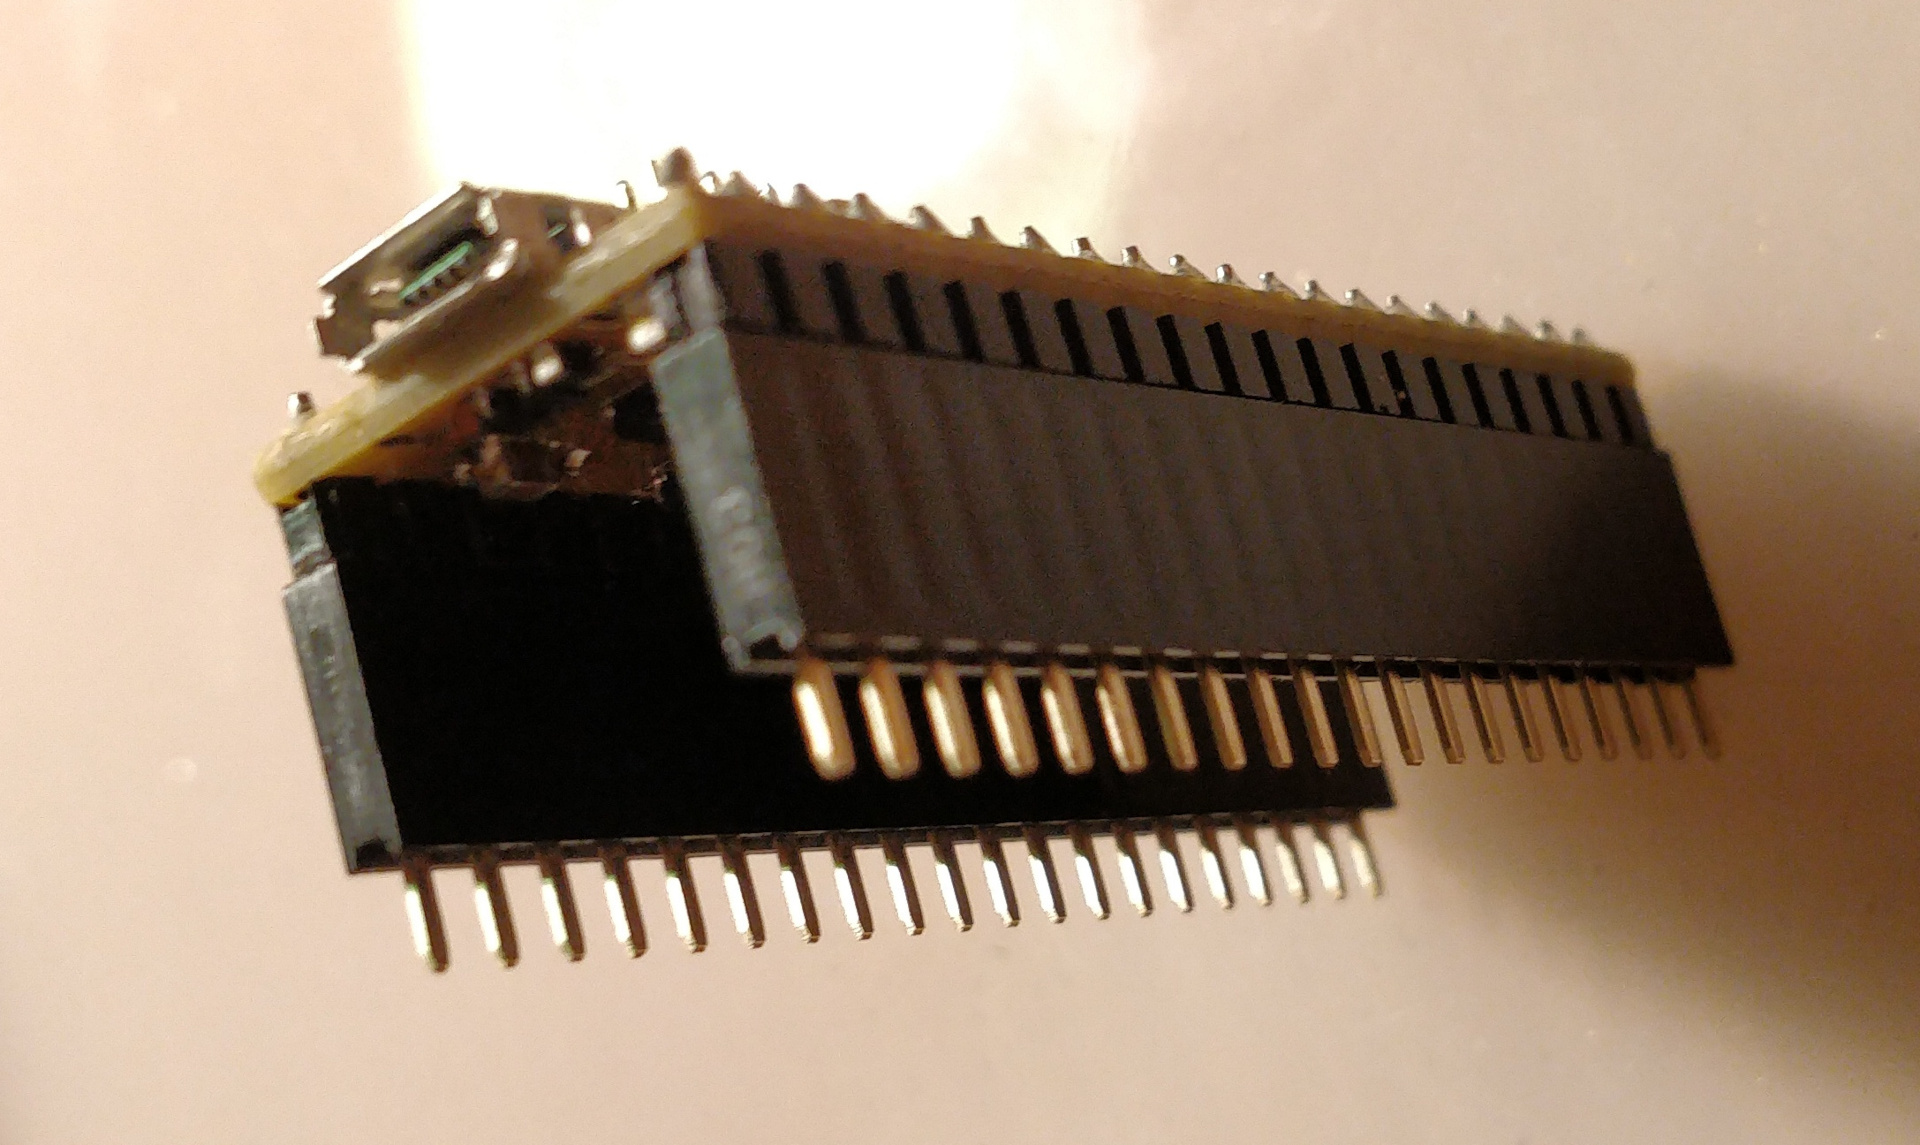
\includegraphics[width=\linewidth]{p04.jpg}
  \caption{Connectors plugged on the Daisy Seed}
  \label{daisy}
\end{figure}

\section{Power}

The next step is to solder on the power connector. Mind its orientation -- if soldered incorrectly, you won't be able to connect the power cable properly.

\begin{enumerate}
  \item Take the shrouded 2\texttimes5 connector and put it on the marked place on the side 1A. Make sure the dent in the connector faces up, as illustrated on the PCB and in figure \ref{connectors}.
  \item Solder all the pins.
\end{enumerate}

\section{Debug (optional)}

The 1\texttimes5 connector is used for firmware debugging and for possible future extensions of the module. This part is optional.

\begin{enumerate}
  \item Put the connector on the marked place on the side 1A. See figure \ref{connectors}.
  \item Solder one of its pins to hold the connector in place.
  \item Make sure the connector is holding right angle to the board, if it needs more alignment, just heat up the pin and fix it.
  \item Once satisfied with the orientation, solder the rest of the pins.
\end{enumerate}

\begin{figure}[p]
  \centering
  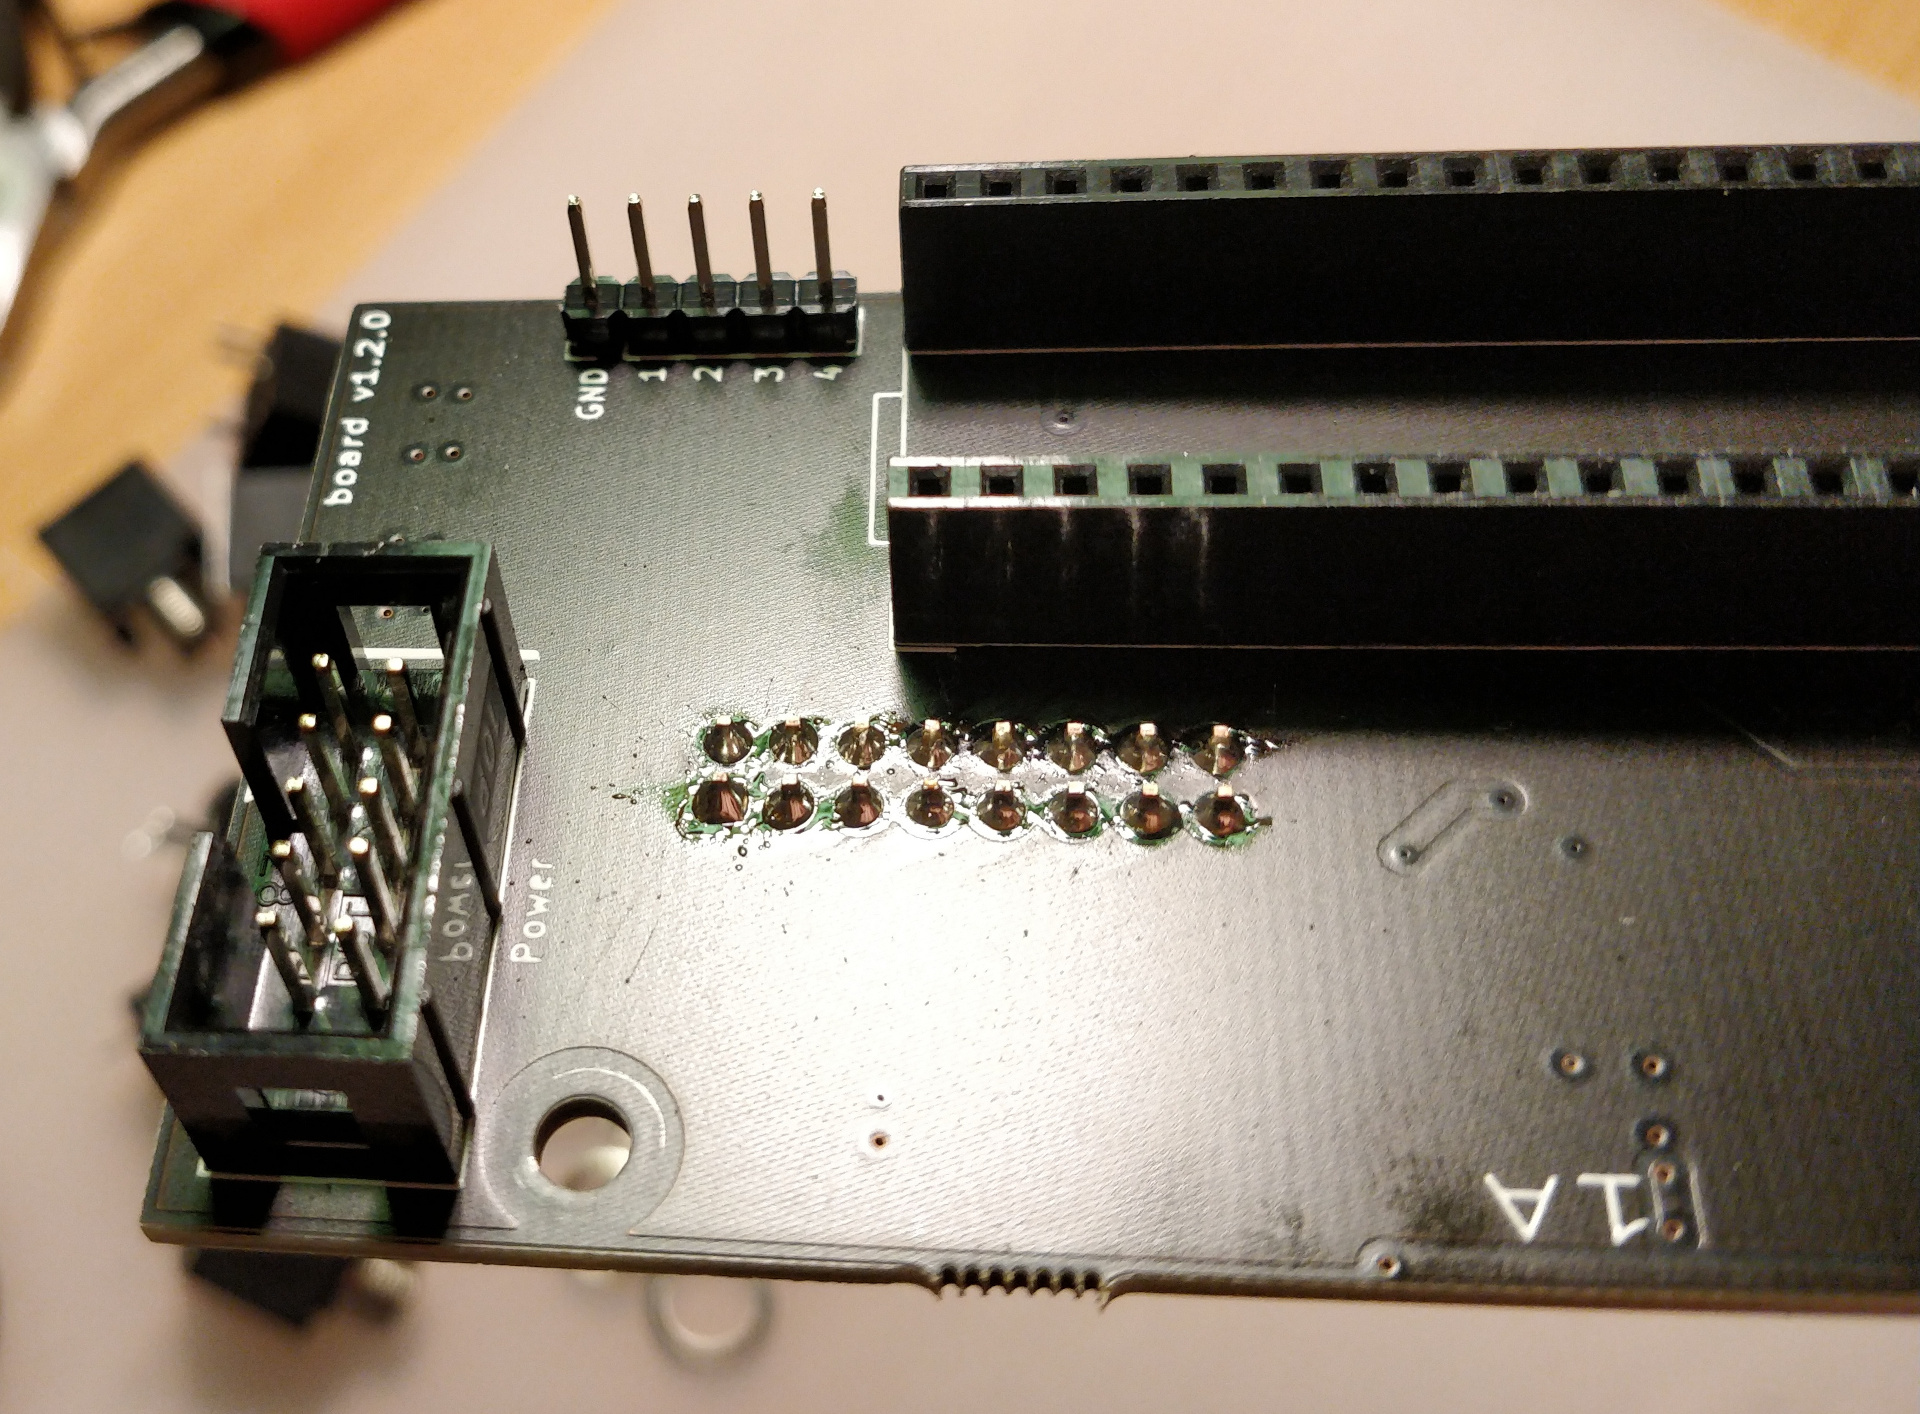
\includegraphics[width=\linewidth]{p05.jpg}
  \caption{Daisy Seed, power and debug connectors}
  \label{connectors}
\end{figure}

\clearpage

\section{Front panel}

Now when all the internal parts are soldered, the last step would be to assemble parts sitting in the front panel.

\begin{enumerate}
  \item Place all potentiometers in the PCB, do not solder them yet. The big legs on sides are used to snap the pot in.
  \item Put all jack sockets into the PCB.
  \item Put LEDs in place. The cathode (shorter leg) goes through the hole closer to the edge, marker with a square pad. See figure \ref{led}.
  \item Snap in the switch. Take care not to bend its leg. Don't push the switch all the way to the PCB. See figure \ref{front components}.
  \item Screw on the standoff on the PCB 2. It should be standing on the side 2A.
  \item Now when all parts are in, carefully put the front panel on them. Be patient aligning all parts so they fit through holes. The switch may be a little problematic, if you see it not getting through, use tweezers to align its bottom part. Don't worry about the LEDs for now.
  \item Put washers on the pots and jacks. See figure \ref{washers}.
  \item Tighten all the potentiometers and jack sockets in place with their nuts. Take care not to scratch the panel. Plastic tools are prefered, steel drivers should also serve well. If you only have pliers, put them in a thick plastic bag. Protect the panel!
  \item Solder all the pots and jacks. Only solder the three smaller terminals of each potentiometer.
  \item Use a masking tape on the portion of the panel with holes for LEDs, see figure \ref{masking}. Push the LEDs against the tape so they are even with the panel surface.
  \item Solder the LEDs. Then snap their legs off.
  \item Use tweezers to align the switch. The button should be holding right angle against the panel, with about 2 mm of it sticking out. Test that the button can be easily clicked and it returns to its resting position.
  \item Once the button is in a satisfying position, solder one of its legs, double check it can be clicked and that it returns, then solder the remaining legs.
\end{enumerate}

\begin{figure}[p]
  \centering
  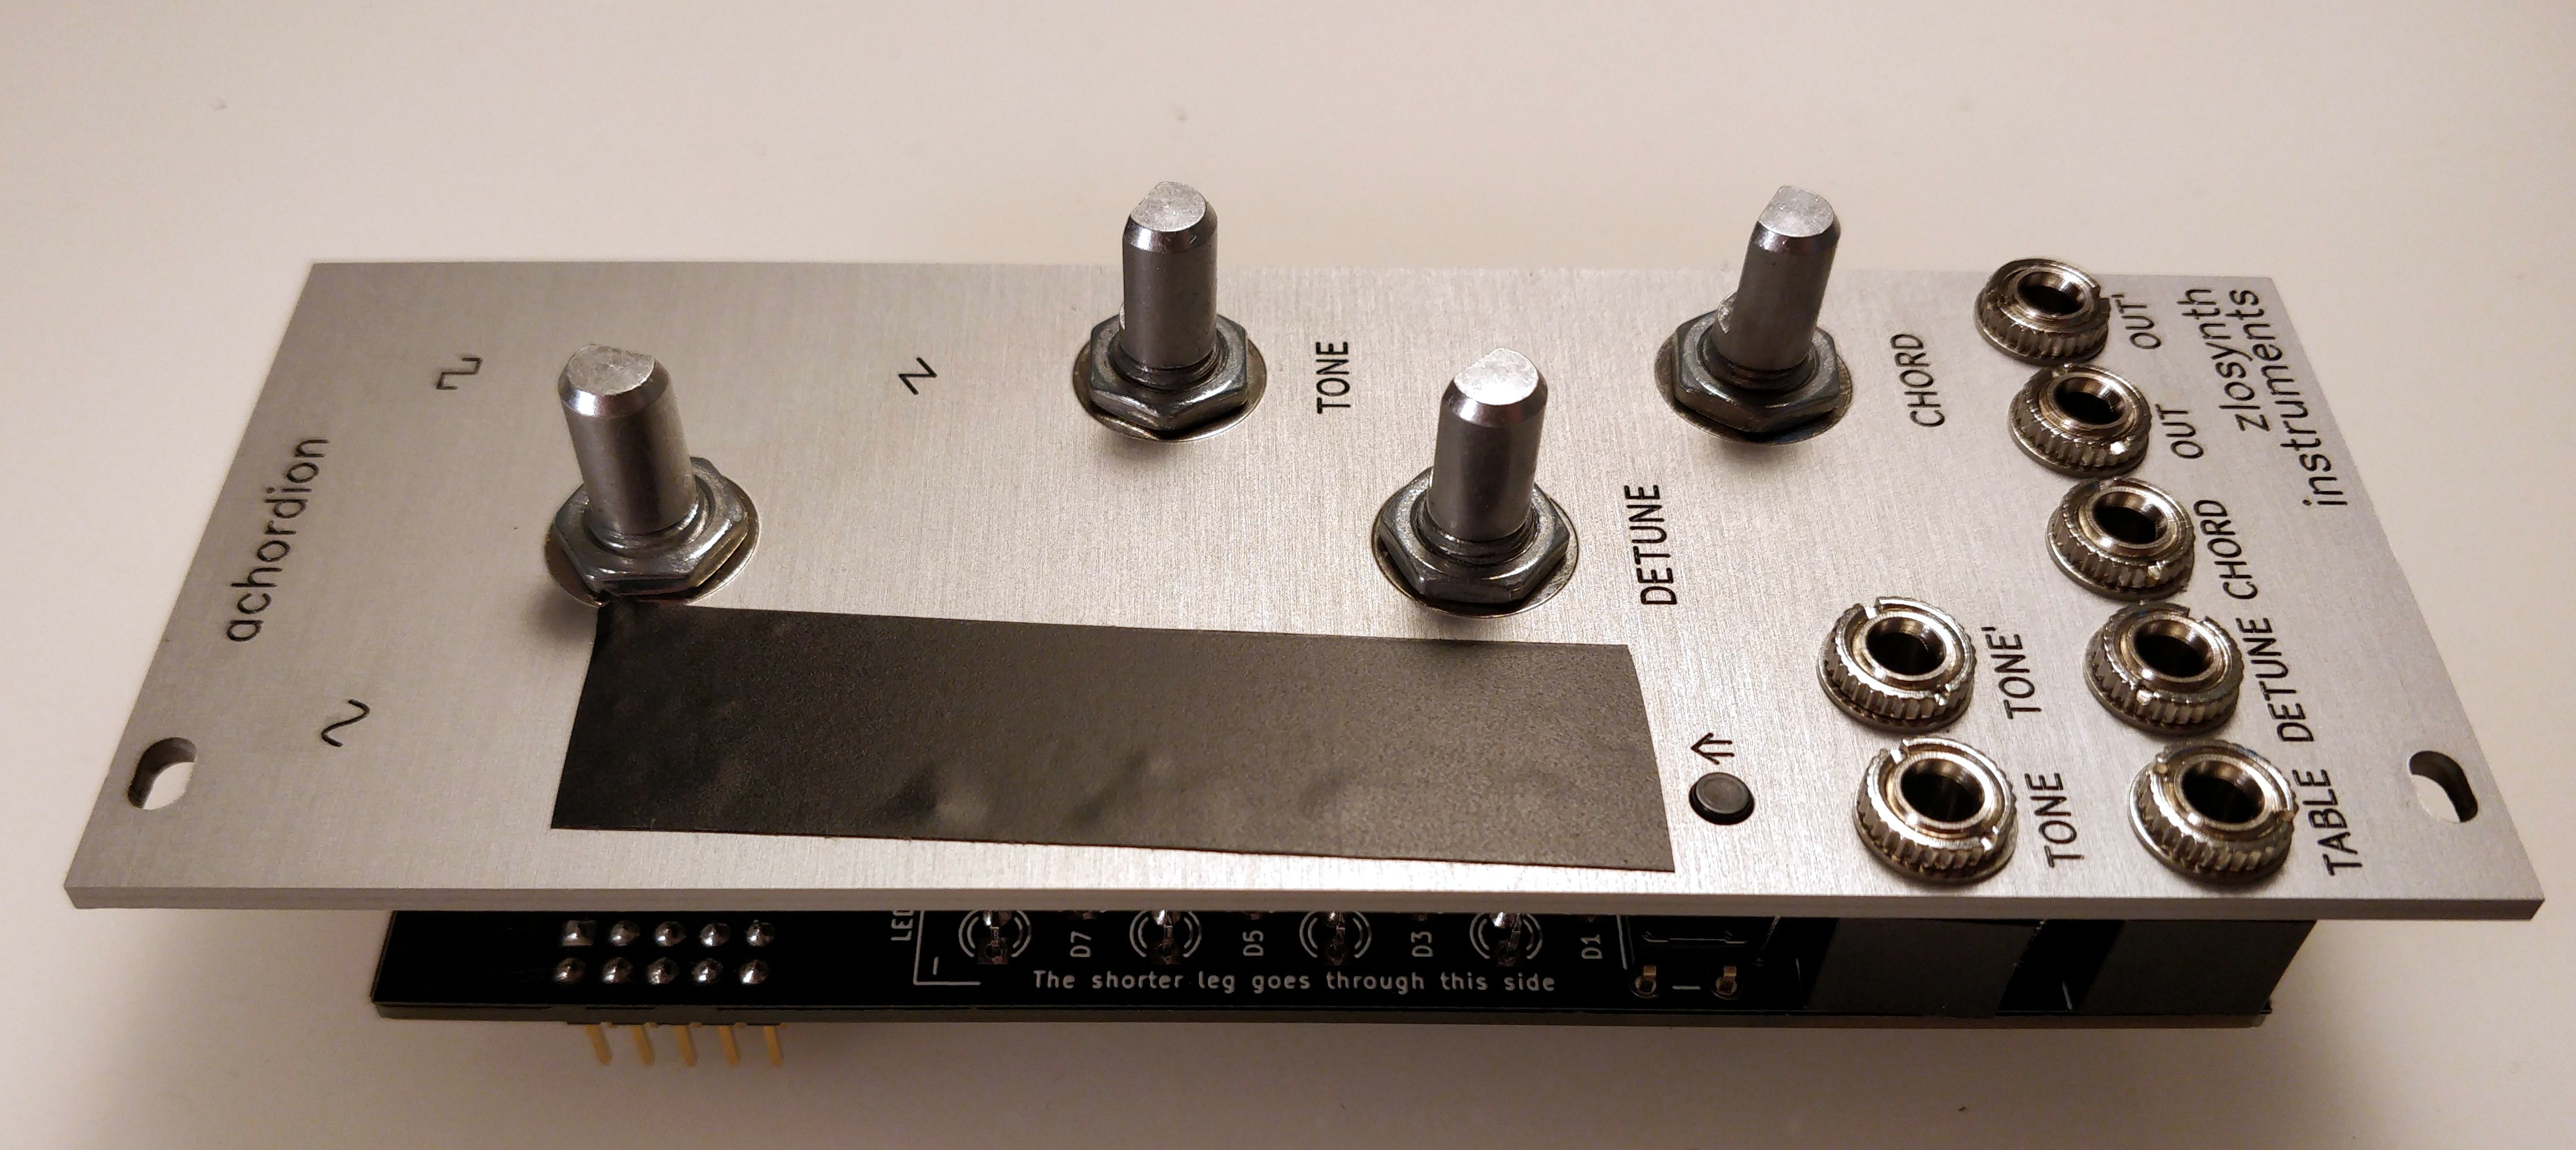
\includegraphics[width=\linewidth]{p06.jpg}
  \caption{Pads of LEDs and the switch}
  \label{led}
\end{figure}

\begin{figure}[p]
  \centering
  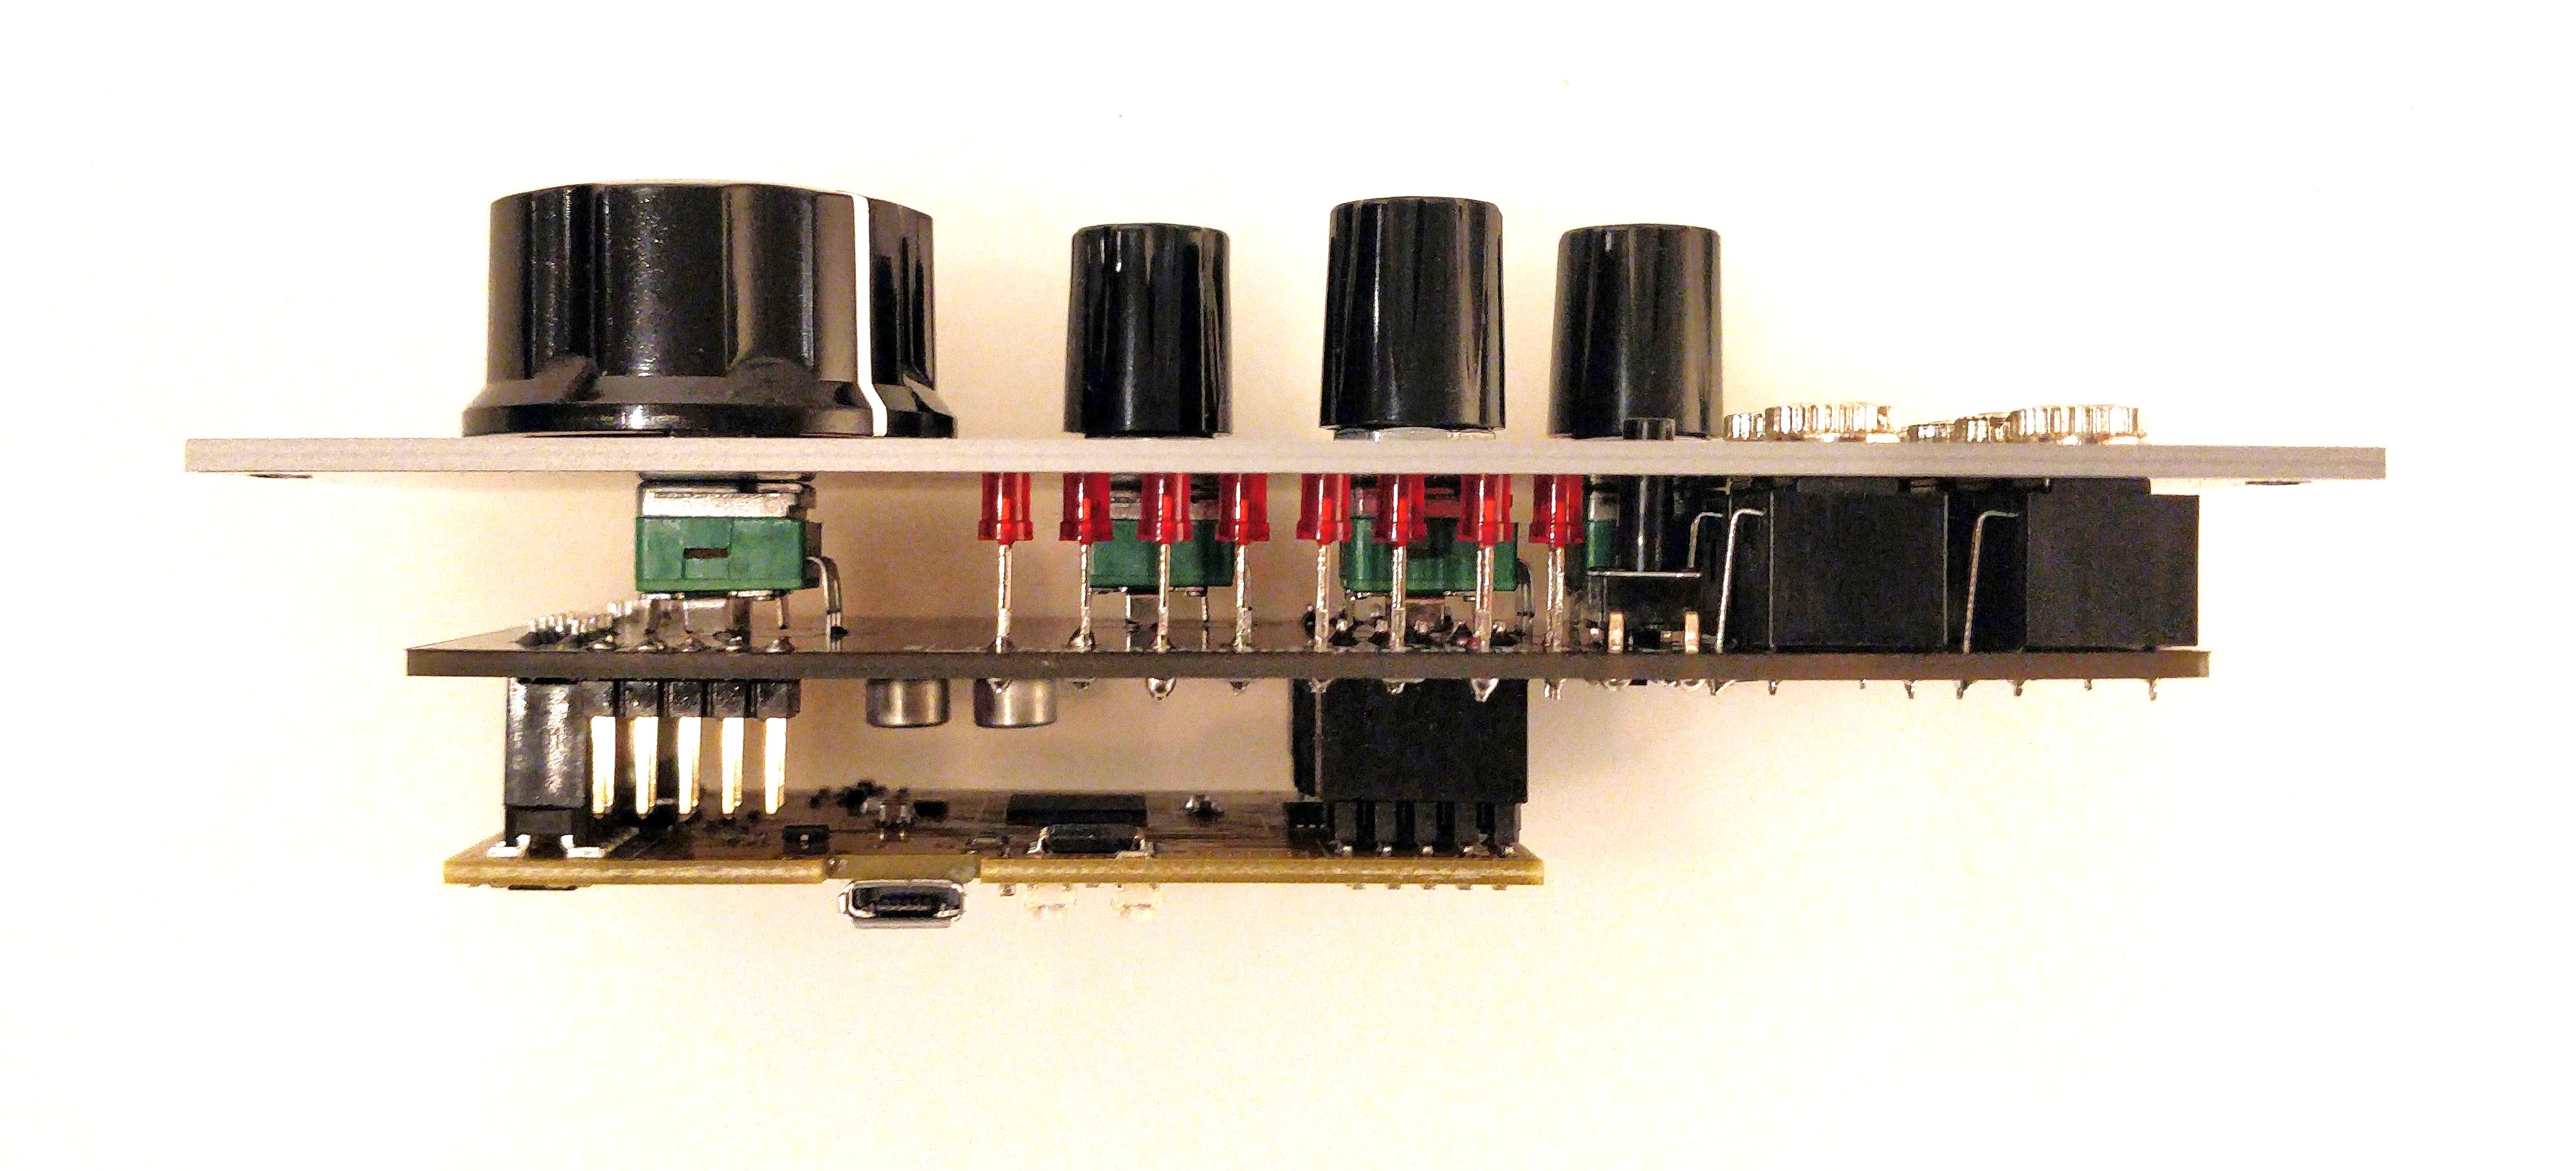
\includegraphics[width=\linewidth]{p07.jpg}
  \caption{Side view with the front components in}
  \label{front components}
\end{figure}

\begin{figure}[p]
  \centering
  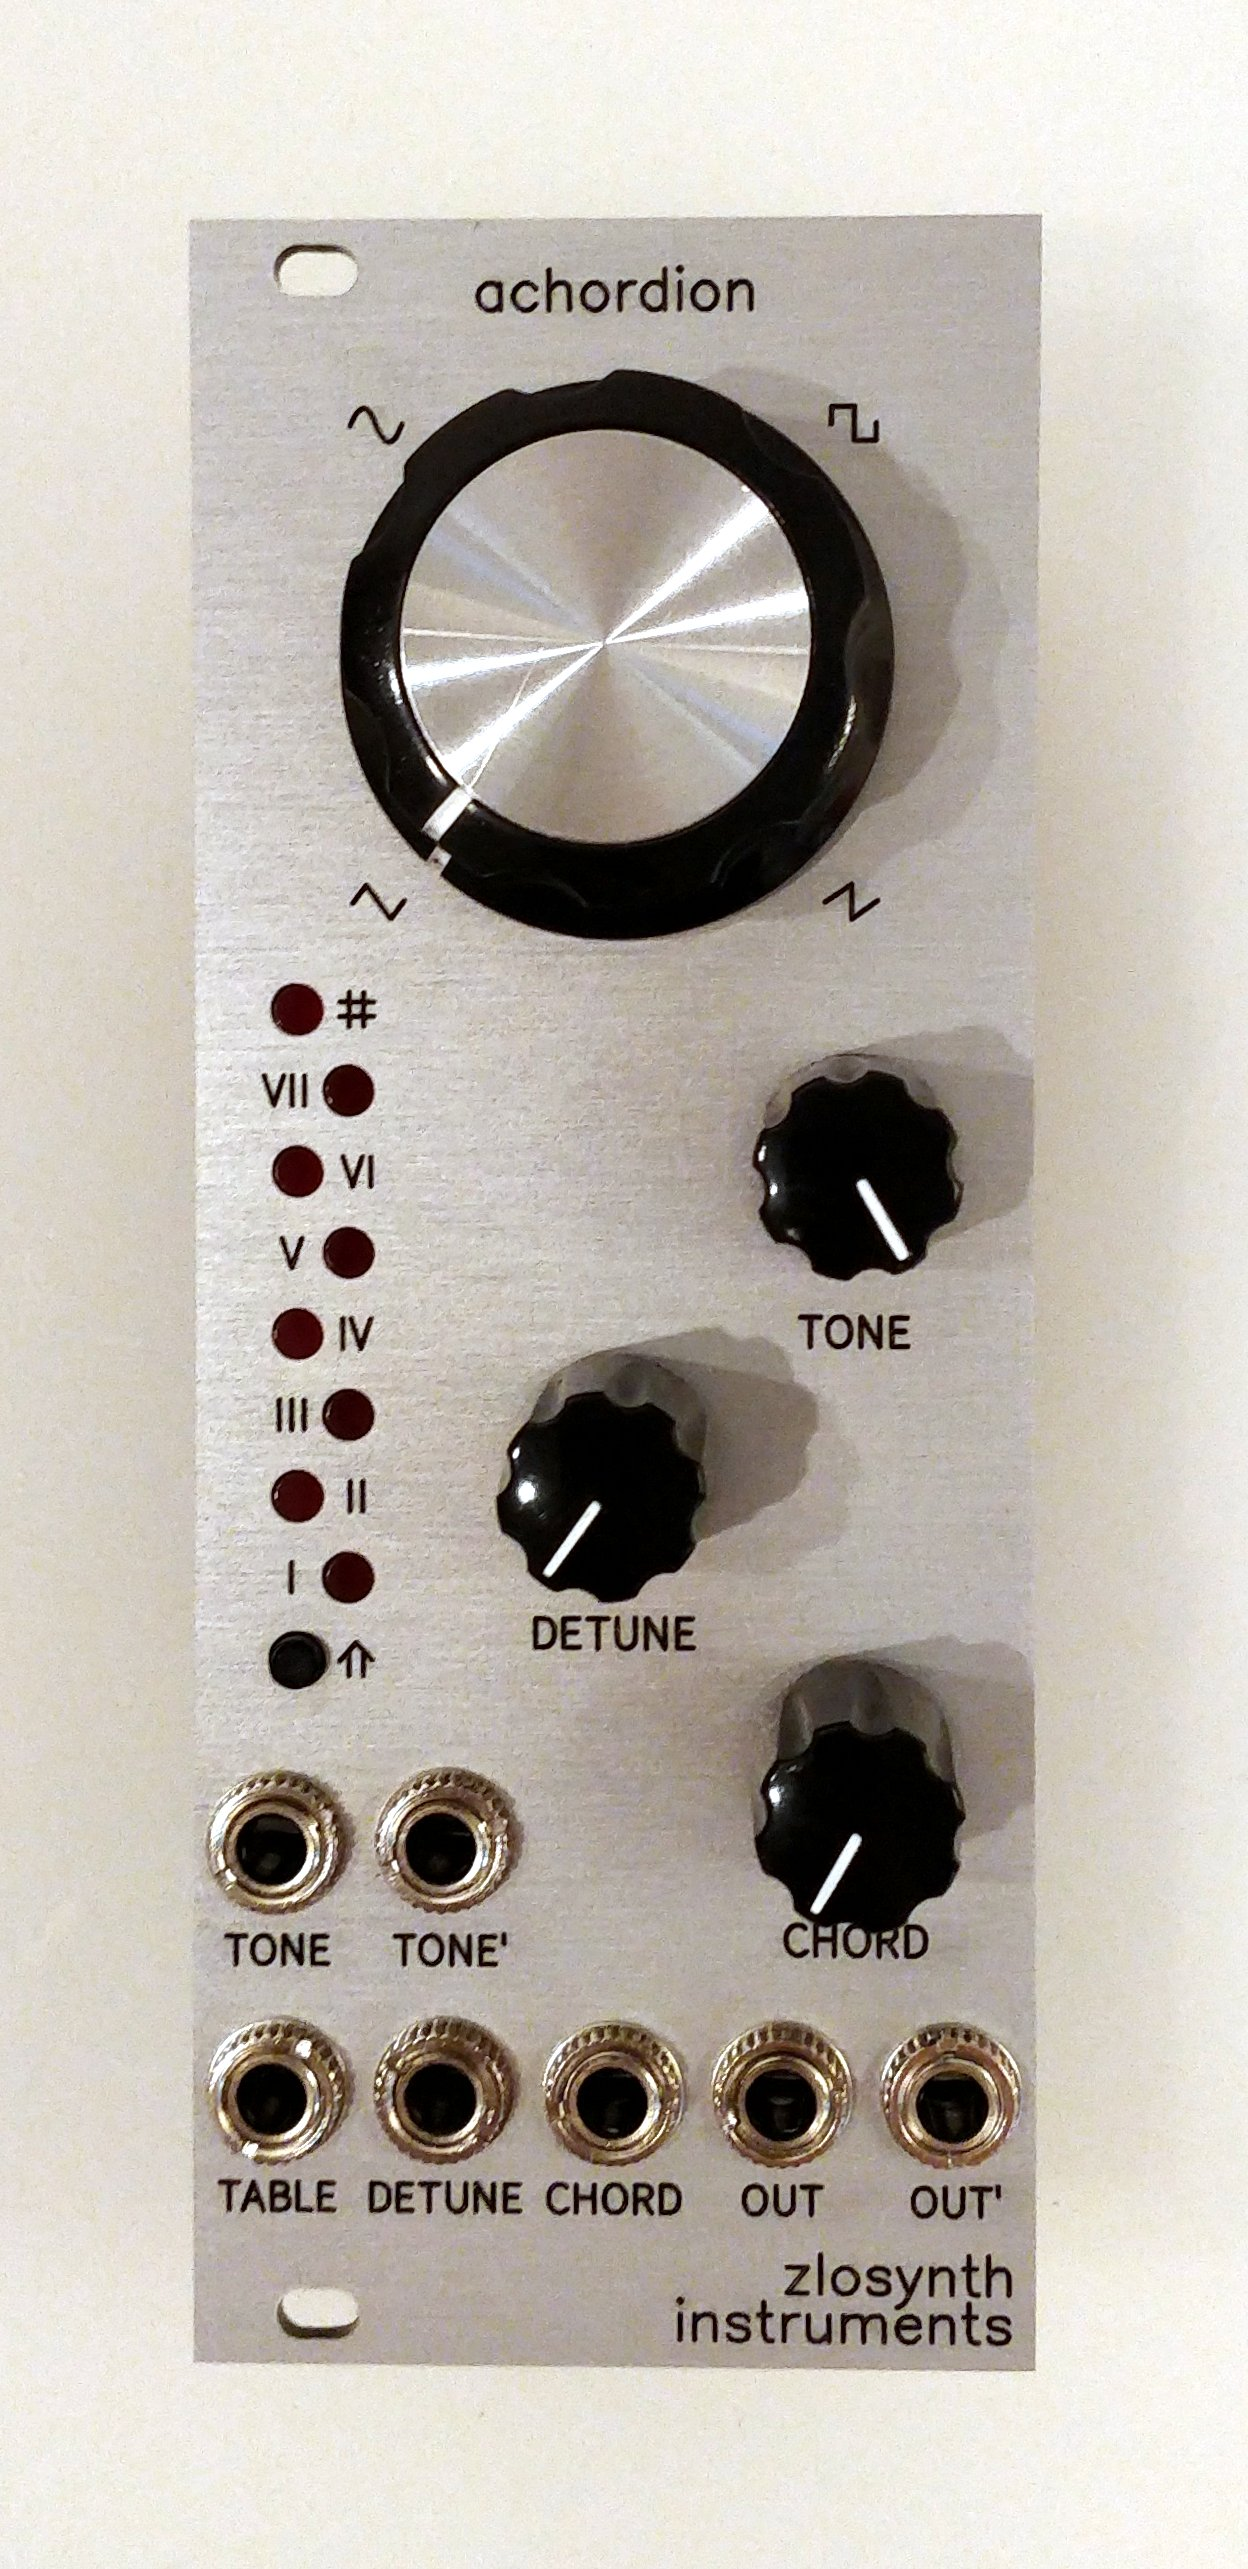
\includegraphics[width=\linewidth]{p08.jpg}
  \caption{Pots and jacks with their washers on}
  \label{washers}
\end{figure}

\begin{figure}[p]
  \centering
  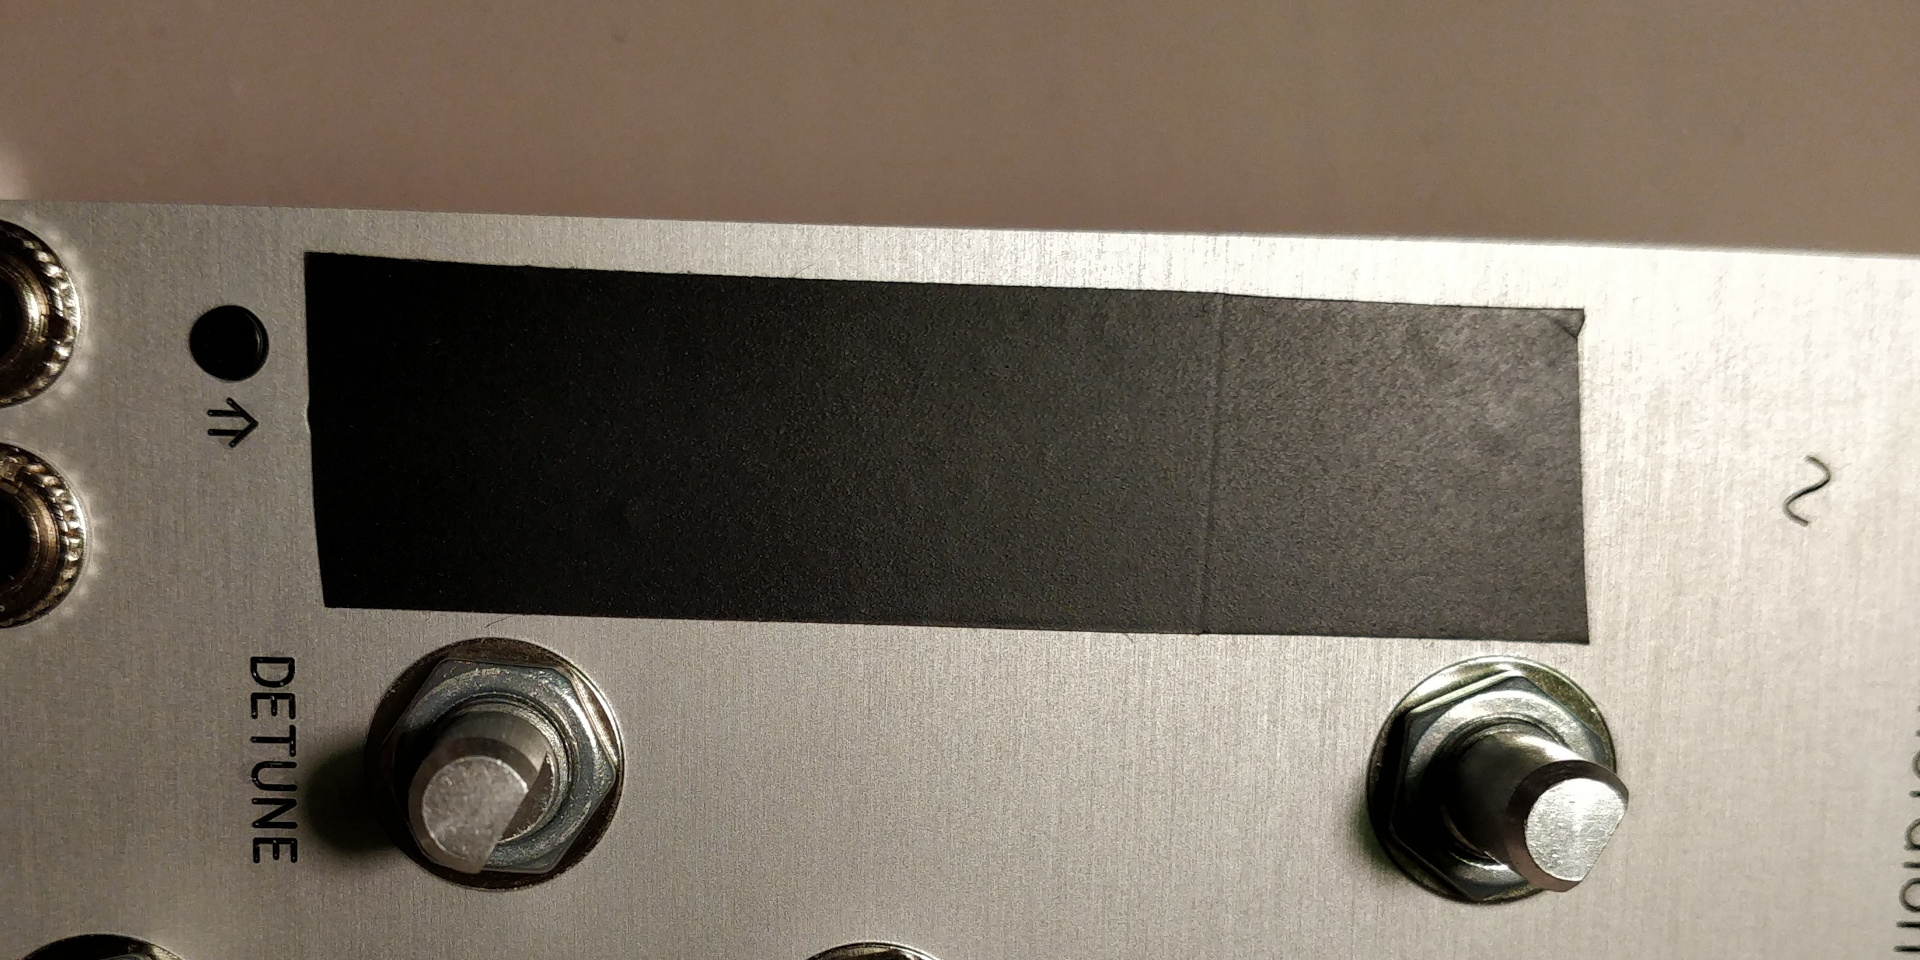
\includegraphics[width=\linewidth]{p09.jpg}
  \caption{Taped LED holes}
  \label{masking}
\end{figure}

\clearpage

\section{Knobs}

You can now put knobs on potentiometers.

\begin{enumerate}
  \item Put the big knob on the topmost potentiometer. Use a small flat screwdriver to tighten the screw of the pot. The screw should be pressing against the flat part of the shaft. Keep some distance between the knob and the panel.
  \item Put smaller black knobs on the remaining pots. Align them with the D-shaped shaft and press them in. You may need to pull them a little bit if you see they are scratching the nut.
\end{enumerate}

\begin{figure}[p]
  \centering
  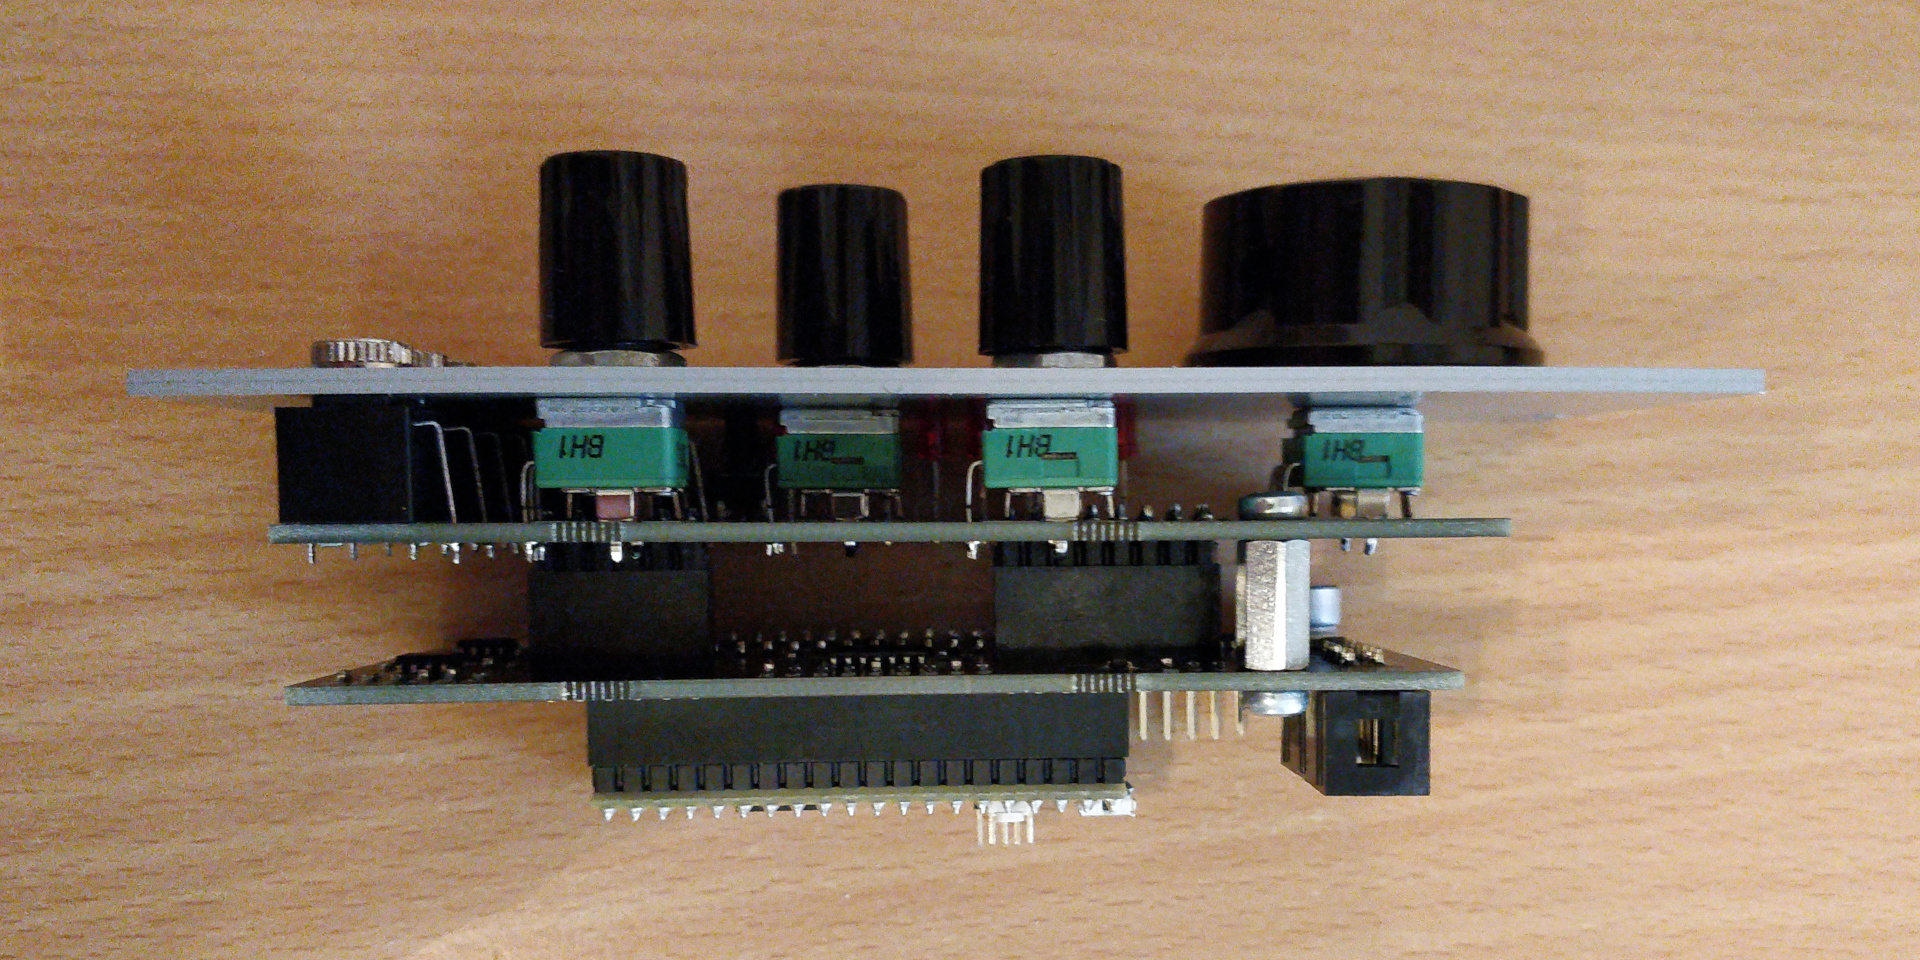
\includegraphics[width=\linewidth]{p11.jpg}
  \caption{Side view of the assembled module}
\end{figure}

\section{Final assembly}

Join all the boards to complete the build.

\begin{enumerate}
  \item Connect PCB 1 and 2 together using their 2\texttimes5 and 2\texttimes8 connectors.
  \item Secure the boards with the standoff screw.
  \item Mount Daisy Seed on its connectors. Mind the orientation.
\end{enumerate}

\begin{figure}[p]
  \centering
  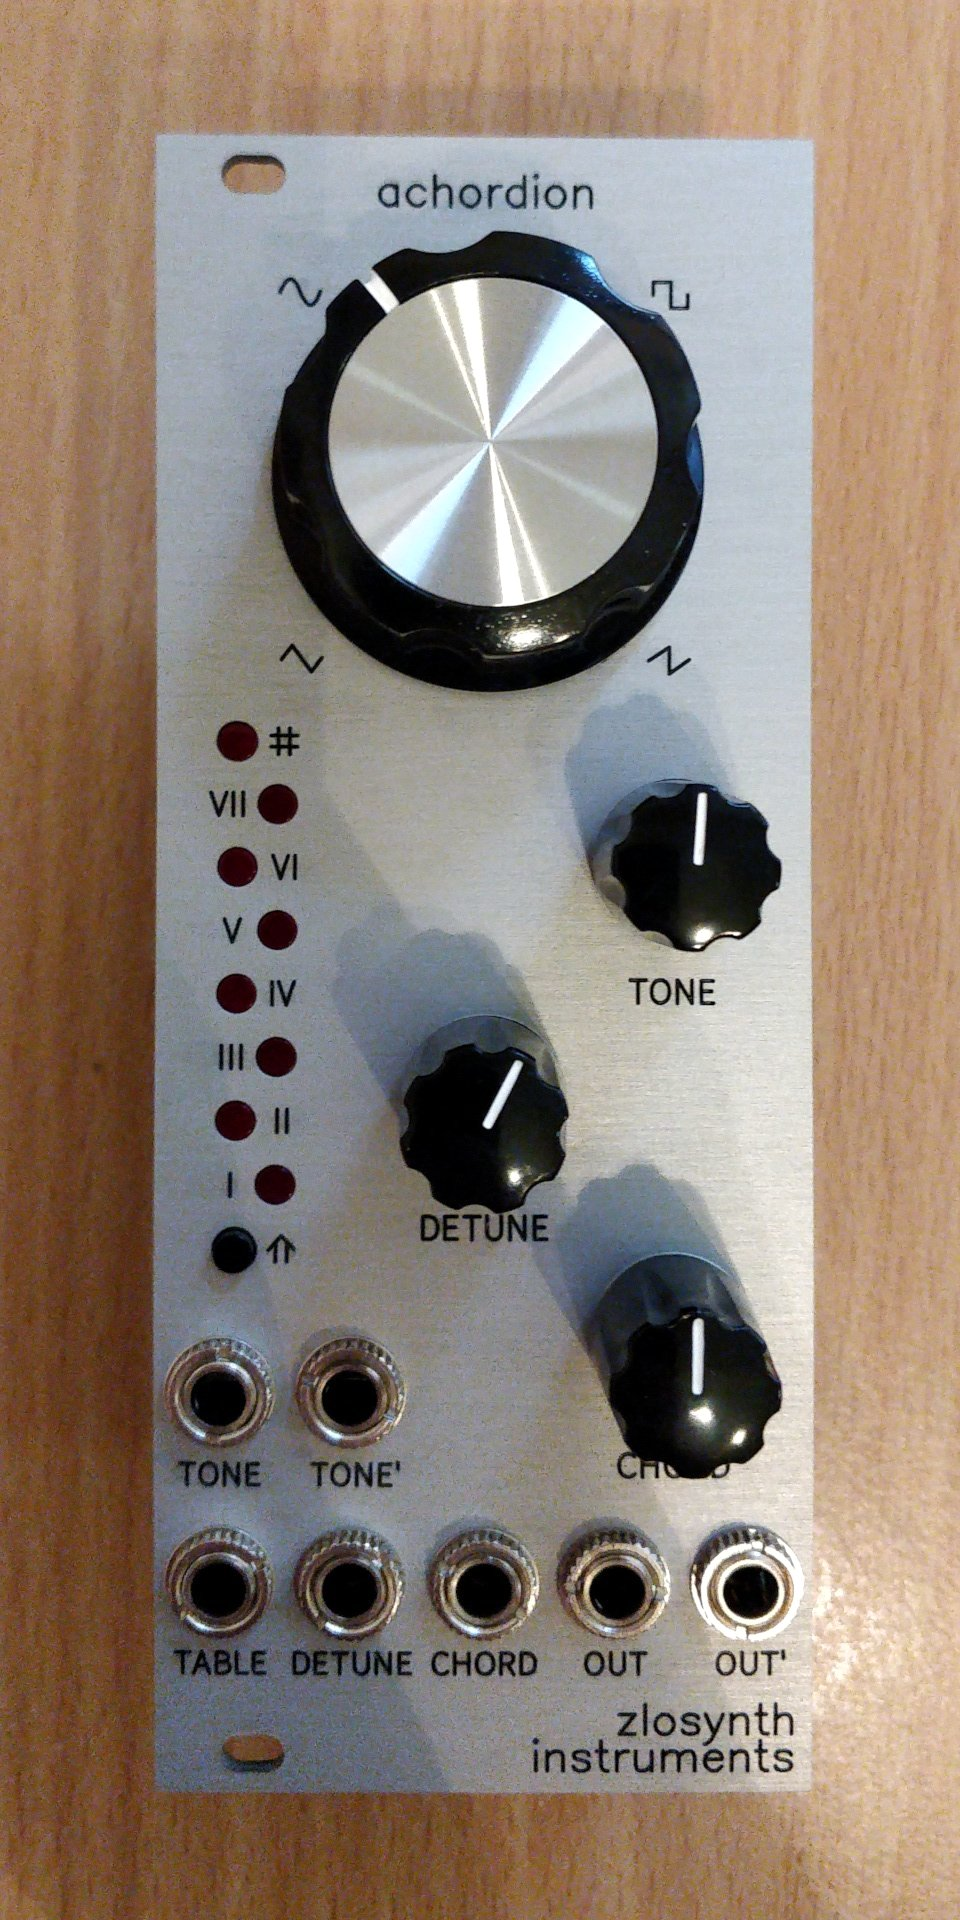
\includegraphics[width=\linewidth]{p12.jpg}
  \caption{Front view of the assembled module}
\end{figure}

\section{Congratulations}

The module is now complete. Have fun!

You can find the user manual on \url{https://zlosynth.com/achordion/user-manual.pdf}.

\end{document}
